$K$-Nearest Neighbours ($K$NN), as the name suggests, is the process of finding $K$ nearest neighbours to a given query point. In this project, $K$NN query is only performed on $2$-dimensional data. We use $\ell_2$ norm as the distance metric. A $K$NN query will be formalised as $\mathcal{K}(\boldsymbol{X})$ where $\boldsymbol{X}\in\mathbb{R}^2$.

\subsubsection{$K$NN query with $K$D-Tree}

\begin{algorithm}[H]
    \SetAlgoLined
    \SetKwInOut{Input}{Input}
    \SetKwInOut{Output}{Output}
    \Input{$K$; Number of nearest neighbour, PointList; Test Points}
    \Output{\texttt{List of $K$ nearest points}}
    \For{$i\gets0$ \KwTo $len(PointList)$}
    {
        \texttt{Start at root}\\
        \texttt{Traverse subtree where the test point $i$ can be added.}\\
        \texttt{Find the leaf; Calculate the distance and store it ($d$).}\\
        \eIf{Points in list < $K$}
            {
                \eIf {Perpendicular distance of Parent with test point <= $d$} 
                    {
                        \texttt{Go down again on the other side} 
                    }
                        {
                            \texttt{Go up another $level$}
                        }
            }
            {
                \texttt{return $K$ nearest list}
            }
        
    }
    \caption{$K$NN Query Algorithm for $K$D-Tree}
    \label{$K$NN_Query_Algorithm_$K$D-Tree}
\end{algorithm}

In algorithm \ref{$K$NN_Query_Algorithm_$K$D-Tree}, we first start with the root to traverse the tree. We find the subtree where the new test point could be added and finally reach the leaf. We calculate the square of the euclidean distance of this point from the test point. We add it to the list and push and pop values from the list depending on the distances we calculate while traversing the tree upwards from here. The main advantage of $K$D-Tree is that we can exploit the tree structure and prune the points we don't think will have distance smaller than the ones we have already calculated. We do this by checking if we should either go up another level or go the other side of the subtree to get a point that could have a distance smaller than the last best calculated distance in the list. 

As a baseline, we first perform $K$NN query with $K$D-tree.

\begin{figure}[htp]
    \centering
    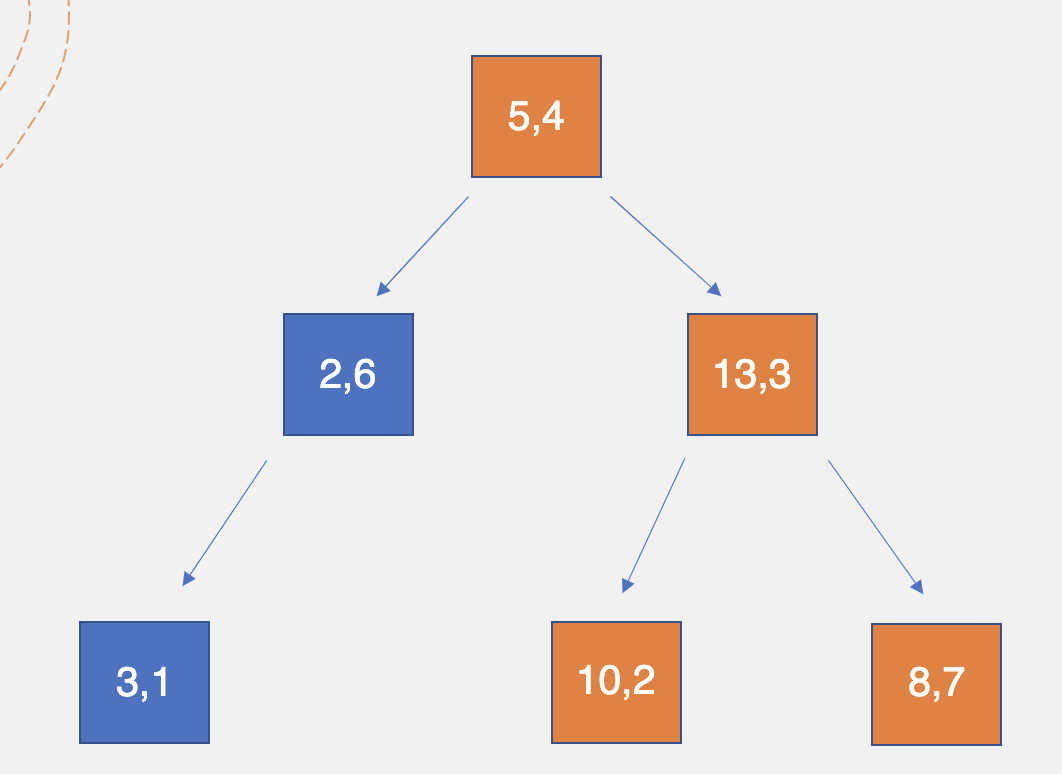
\includegraphics[width=0.4\textwidth]{graphs/KD-Tree_KNN_Tree.png}
    \caption{$K$D-Tree for KNN Query}
    \label{fig:$K$D-Tree_for_KNN Query}
\end{figure}

\begin{figure}[htp]
    \centering
    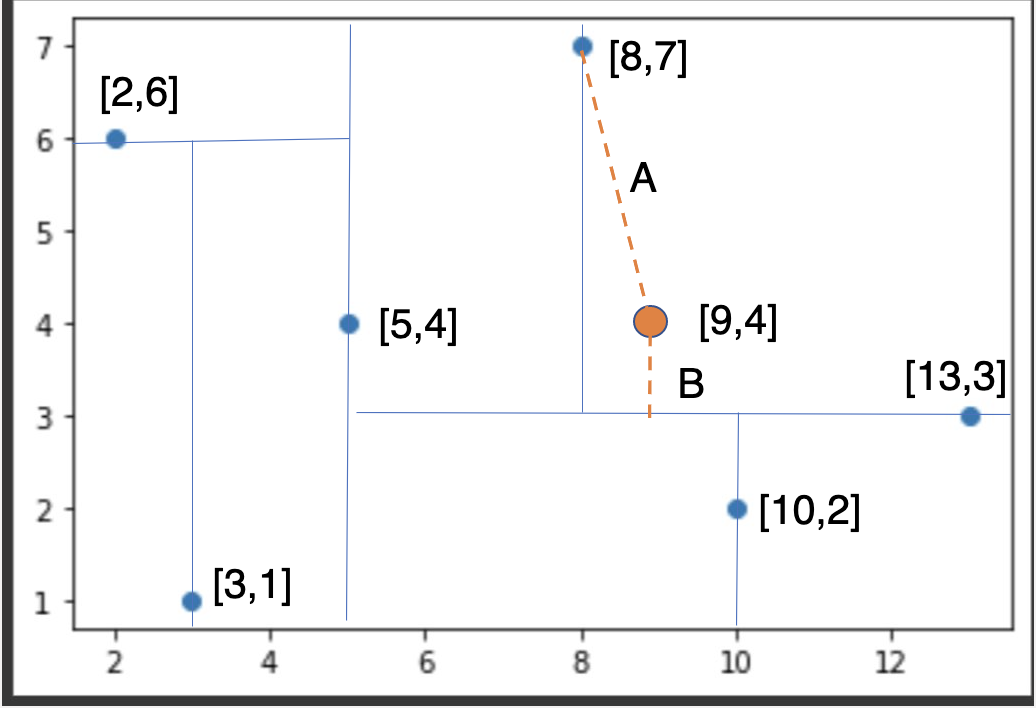
\includegraphics[width=0.6\textwidth]{graphs/KD-Tree_KNN_plot.png}
    \caption{$K$D-Tree KNN Plot on 2-dimentional plane}
    \label{fig:KD_Tree_KNN_Plot}
\end{figure}


\begin{mscexample}
	For example, we have Point list as\\ $((5,4),(2,6),(13,3),(8,7),(3,1),(10,2))]$ 
	
	\textbf{test point} $(9,4)$, we will have a tree structure as shown in \ref{fig:$K$D-Tree_for_KNN Query} and it's plot on $2$-dimensional plane is shown in \ref{fig:KD_Tree_KNN_Plot}. \\
	In fig \ref{fig:KD_Tree_KNN_Plot} we can see that although point $(8,7)$ is the leaf we will reach when we traverse the tree to search where test point $(9,4)$ can be added, it is not in fact the nearest point to the test point. \\
	In this case if we want to look for $4$ nearest neighbour, we will first traverse to $(8,7)$ and then make a decision weather to traverse to the other side of the subtree to point $(10,2)$. We decide this by checking the perpendicular distance of $(13,3)$ with test point $(9,4)$ and compare this with the distance of $(8,7)$ and test point $(9,4)$. We do this to verify if there is even a possibility to find a point smaller than the last best distance on the other side of the subtree. Since the perpendicular distance is smaller than the best calculated distance we will check the distance of test point $(9,4)$ and $(10,2)$ on the other side of the subtree ($A > B$). This distance in our case is indeed smaller than the best calculated distance of test point $(9,4)$ with $(8,7)$ so far and so point $(10,2)$ will be added to the list.\\
	Similarly, we traverse until we have $K$ nearest neighbour to the test point in the list.
\end{mscexample}



\subsubsection{$K$NN Query with LISA}
%TODO: What does this paragraph mean?
%We do not know the analytical representation of shards, as we use machine learning model $ \mathcal{SP}$ to generate shards. Thus, 
It is difficult to apply traditional $K$NN query pruning strategies applicable for $K$D-Trees, to LISA model as we don't maintain a tree like structure in LISA. Shard boundaries are learned per mapped interval and no data structure is maintained to refer to shards in adjacent mapped intervals.The key idea in the $K$NN query is to convert it into a range query by estimating an appropriate query range.The query range is augmented if less than K neighbors are found in a range query.

Consider a query point $q_{knn}=(x_{0},x_{1})$, let $x^{'} \in V$ be the $K$th nearest key to $x$ in database at a distance value $\delta = \| x^{'}-q_{knn}\|_{2} $. Lets define $ \mathcal{Q}(q_{knn},\delta) \triangleq [x_{0}-\delta, x_{0}+\delta) \times[x_{1}-\delta, x_{1}+\delta)$ and $\mathcal{B}(q_{knn}, \delta)  \triangleq \{p \in V \mid \| q_{knn}-p\|_{2} \leq \delta \} $. We can create a query rectangle $qr =  \mathcal{Q}(q_{knn}, \delta + \epsilon)$ where $\epsilon \rightarrow 0$. As shown in Fig. \ref{fig:KNN_Query_Lisa}, K nearest keys to $q_{knn}$ are all in $\mathcal{B}(q_{knn}, \delta)$ and thus in $\mathcal{Q}$. $K$NN query can be solved using the range query if we can estimate an appropriate distance bound $\delta$ for every query point.

\begin{figure*}[t]
    \centering
    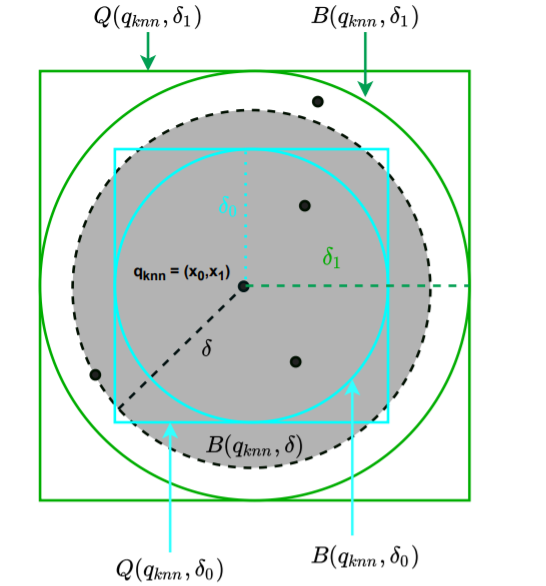
\includegraphics[width=0.7\textwidth]{graphs/KNN_Query_Lisa.png}
    \caption{KNN Query Implementation in Lisa(K=3)\\
    1)$q_{knn}$ represents the query point, $ \mathcal{Q}(x,\delta) \triangleq [x_{0}-\delta, x_{0}+\delta) \times[x_{1}-\delta, x_{1}+\delta)$, represents query rectangle and $ \mathcal{B}(x, \delta)$ represents the key space at distance $\delta$ containing K nearest keys.\\
    2)KNN query can be solved by range query if we can estimate an appropriate distance bound $\delta$ for every query point\\
    }
    \label{fig:KNN_Query_Lisa}
\end{figure*}
In our experiments, we find the $\delta$ empirically. We try with different values of $\delta$ and choose the one for which we get the best results. 